\documentclass[11pt]{article}

%% MinionPro fonts 
%\usepackage[lf]{MinionPro}
%\usepackage{MnSymbol}
\usepackage{microtype}

%% Margins
\usepackage{geometry}
\geometry{verbose,letterpaper,tmargin=1in,bmargin=1in,lmargin=1in,rmargin=1in}

%% Other packages
\usepackage{amsmath}
\usepackage{amsthm}
\usepackage[shortlabels]{enumitem}
\usepackage{titlesec}
\usepackage{soul}
\usepackage{tikz}
\usepackage{mathtools}
\usepackage{pgfplots}
\usepackage{tikz-3dplot}
\usepackage{algorithmic}
\usepackage{optprog}
\usepackage[export]{adjustbox}
\usepackage{tcolorbox}
\usepackage{amsfonts}


%% Paragraph style settings
\setlength{\parskip}{\medskipamount}
\setlength{\parindent}{0pt}

%% Change itemize bullets
\renewcommand{\labelitemi}{$\bullet$}
\renewcommand{\labelitemii}{$\circ$}
\renewcommand{\labelitemiii}{$\diamond$}
\renewcommand{\labelitemiv}{$\cdot$}

%% Colors
\definecolor{rred}{RGB}{204,0,0}
\definecolor{ggreen}{RGB}{0,145,0}
\definecolor{yyellow}{RGB}{255,185,0}
\definecolor{bblue}{rgb}{0.2,0.2,0.7}
\definecolor{ggray}{RGB}{190,190,190}
\definecolor{ppurple}{RGB}{160,32,240}
\definecolor{oorange}{RGB}{255,165,0}

%% Shrink section fonts
\titleformat*{\section}{\normalsize\bf}
\titleformat*{\subsection}{\normalsize\bf}
\titleformat*{\subsubsection}{\normalsize\it}

% %% Compress the spacing around section titles
\titlespacing*{\section}{0pt}{1.5ex}{0.75ex}
\titlespacing*{\subsection}{0pt}{1ex}{0.5ex}
\titlespacing*{\subsubsection}{0pt}{1ex}{0.5ex}

%% amsthm settings
\theoremstyle{definition}
\newtheorem{problem}{Problem}
\newtheorem{example}{Example}
\newtheorem*{theorem}{Theorem}
\newtheorem*{bigthm}{Big Theorem}
\newtheorem*{biggerthm}{Bigger Theorem}
\newtheorem*{bigcor1}{Big Corollary 1}
\newtheorem*{bigcor2}{Big Corollary 2}

%% tikz settings
\usetikzlibrary{calc}
\usetikzlibrary{patterns}
\usetikzlibrary{decorations}
\usepgfplotslibrary{polar}

%% algorithmic setup
\algsetup{linenodelimiter=}
\renewcommand{\algorithmiccomment}[1]{\quad// #1}
\renewcommand{\algorithmicrequire}{\emph{Input:}}
\renewcommand{\algorithmicensure}{\emph{Output:}}

%% Answer box macros
%% \answerbox{alignment}{width}{height}
\newcommand{\answerbox}[3]{%
  \fbox{%
    \begin{minipage}[#1]{#2}
      \hfill\vspace{#3}
    \end{minipage}
  }
}

%% \answerboxfull{alignment}{height}
\newcommand{\answerboxfull}[2]{%
  \answerbox{#1}{6.38in}{#2} 
}

%% \answerboxone{alignment}{height} -- for first-level bullet
\newcommand{\answerboxone}[2]{%
  \answerbox{#1}{6.0in}{#2} 
}

%% \answerboxtwo{alignment}{height} -- for second-level bullet
\newcommand{\answerboxtwo}[2]{%
  \answerbox{#1}{5.8in}{#2}
}

%% special boxes
\newcommand{\wordbox}{\answerbox{c}{1.2in}{.7cm}}
\newcommand{\catbox}{\answerbox{c}{.5in}{.7cm}}
\newcommand{\letterbox}{\answerbox{c}{.7cm}{.7cm}}

%% Miscellaneous macros
\newcommand{\tstack}[1]{\begin{multlined}[t] #1 \end{multlined}}
\newcommand{\cstack}[1]{\begin{multlined}[c] #1 \end{multlined}}
\newcommand{\ccite}[1]{\only<presentation>{{\scriptsize\color{gray} #1}}\only<article>{{\small [#1]}}}
\newcommand{\grad}{\nabla}
\newcommand{\ra}{\ensuremath{\rightarrow}~}
\newcommand{\maximize}{\text{maximize}}
\newcommand{\minimize}{\text{minimize}}
\newcommand{\subjectto}{\text{subject to}}
\newcommand{\trans}{\mathsf{T}}
\newcommand{\bb}{\mathbf{b}}
\newcommand{\bx}{\mathbf{x}}
\newcommand{\bc}{\mathbf{c}}
\newcommand{\bd}{\mathbf{d}}
\newcommand{\blu}{\color{blue}}


%% LP format
%    \begin{align*}
%      \maximize \quad & \mathbf{c}^{\trans} \mathbf{x}\\
%      \subjectto \quad & A \mathbf{x} = \mathbf{b}\\
%                       & \mathbf{x} \ge \mathbf{0}
%    \end{align*}


%% Redefine maketitle
\makeatletter
\renewcommand{\maketitle}{
  \noindent SA405 

  \begin{center}\Large{\textbf{\@title}}\end{center}
}
\makeatother

%% ----- Begin document ----- %%
\begin{document}
\title{HW2: Intro to Network Models-Solution}

\maketitle

\textbf{1.} Graham Krackers has 3 plants where it produces (you guessed it) graham crackers that it then ships to 5 warehouses. The table below gives the plant and warehouse locations as well as the cost to ship between each plant and warehouse.

\begin{figure}[h!!!]
    \centering
    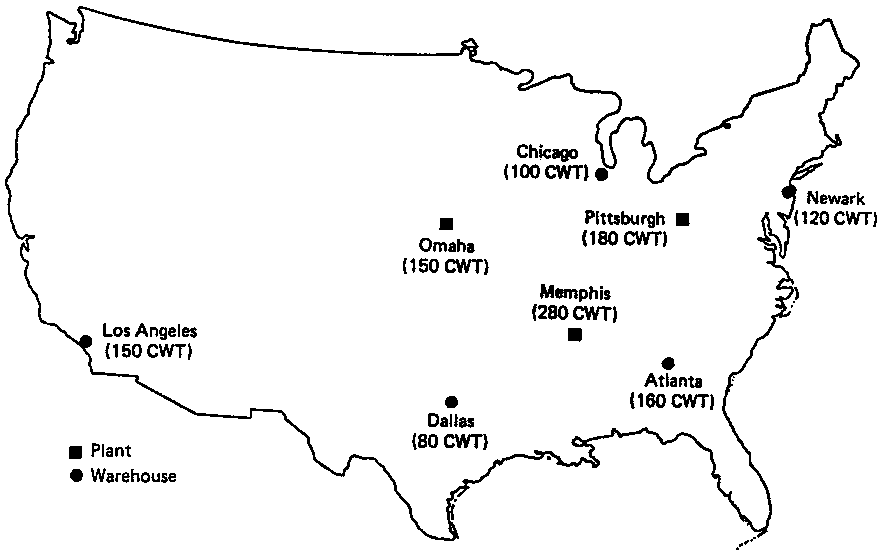
\includegraphics[width=4.3in]{map}\\
    \caption{Locations of Graham Krackers’ plants and warehouses}
\end{figure}

\begin{center}\begin{tabular}{|ccccccc|}\hline
  \$/ton   & Warehouse 1 & Warehouse 2 & Warehouse 3 & Warehouse 4 & Warehouse 5 &            \\
           &   (Newark) &  (Chicago) &  (Atlanta) &   (Dallas) & (Los Angeles) &   Supply   \\\cline{2-7}
   Plant 1 & \multicolumn{1}{|c|}{4} & \multicolumn{1}{|c|}{6} & \multicolumn{1}{|c|}{5} & \multicolumn{1}{|c|}{12} & \multicolumn{1}{|c|}{19} &    180 tons \\
(Pittsburgh) & \multicolumn{1}{|c|}{} & \multicolumn{1}{|c|}{} & \multicolumn{1}{|c|}{} & \multicolumn{1}{|c|}{} & \multicolumn{1}{|c|}{} &            \\ \cline{2-6}
   Plant 2 & \multicolumn{1}{|c|}{10} & \multicolumn{1}{|c|}{4} & \multicolumn{1}{|c|}{8} & \multicolumn{1}{|c|}{5} & \multicolumn{1}{|c|}{14} &    280 tons \\
 (Memphis) & \multicolumn{1}{|c|}{} & \multicolumn{1}{|c|}{} & \multicolumn{1}{|c|}{} & \multicolumn{1}{|c|}{} & \multicolumn{1}{|c|}{} &            \\ \cline{2-6}
   Plant 3 & \multicolumn{1}{|c|}{13} & \multicolumn{1}{|c|}{9} & \multicolumn{1}{|c|}{3} & \multicolumn{1}{|c|}{6} & \multicolumn{1}{|c|}{10} &    150 tons \\
   (Omaha) & \multicolumn{1}{|c|}{} & \multicolumn{1}{|c|}{} & \multicolumn{1}{|c|}{} & \multicolumn{1}{|c|}{} & \multicolumn{1}{|c|}{} &            \\ \cline{1-6}
   Demand &    120 tons &    100 tons &    160 tons &     80 tons &    150 tons &            \\ \hline
\end{tabular}\end{center}

\begin{enumerate}
\item[a)] Draw the network diagram for this problem.

\begin{center}
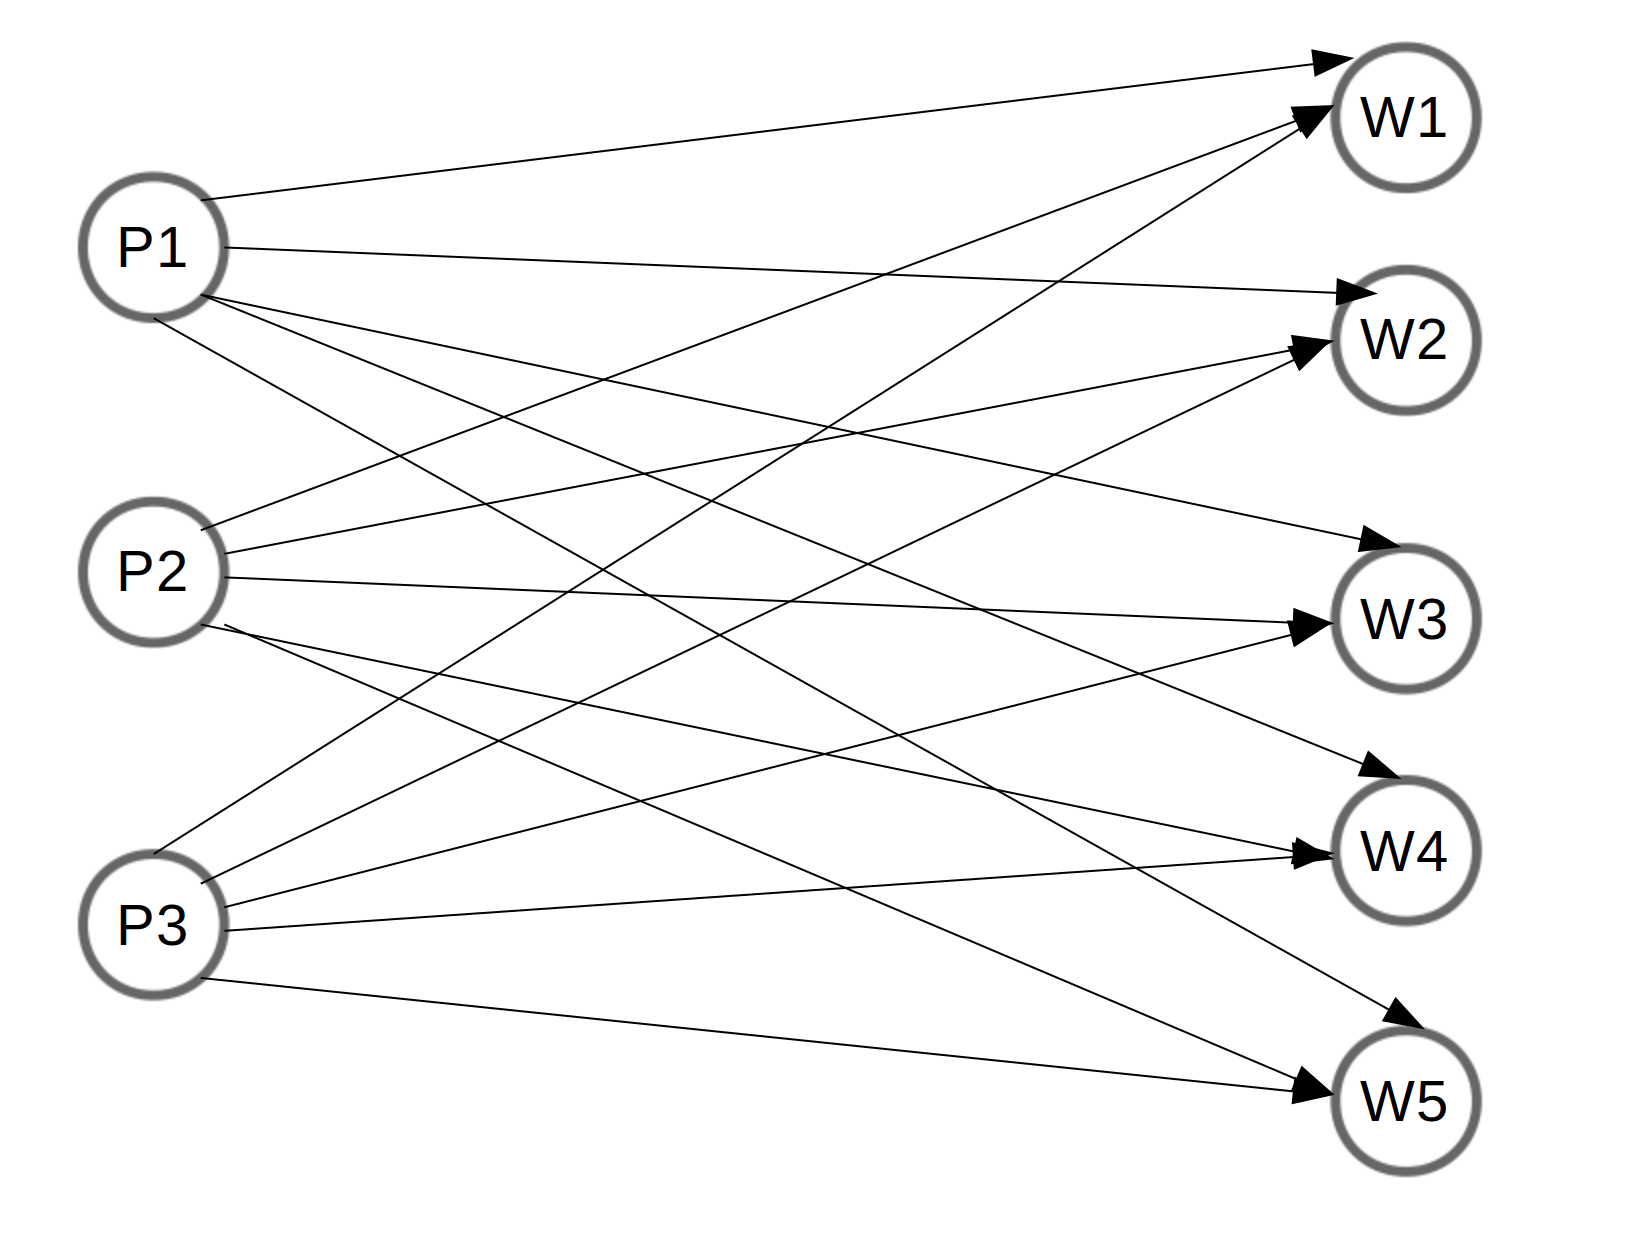
\includegraphics[width=0.9\textwidth]{Prob1.png}
\end{center}

\item[b)] Formulate a concrete model that would allow Graham Krackers to satisfy demand of the warehouses at minimum cost.

{\blu

\textbf{\underline{Decision Variables}}

Let $x_{1,1}$ be the number of crackers sent from plant 1 to warehouse 1

Let $x_{1,2}$ be the number of crackers sent from plant 1 to warehouse 2 

$\vdots$

Let $x_{3,5}$ be the number of crackers sent from plant 3 to warehouse 5

\textbf{\underline{Objective Function}}

\[
\text{min cost: } 4 x_{1,1} + 6 x_{1,2} + \cdots + 10 x_{3,5}
\]

\textbf{\underline{Constraints}}

\begin{optprog*}
st & x_{1,1} + x_{1,2} + x_{1,3} + x_{1,4} + x_{1,5} & \leq & 180 & \text{(supply of plant 1)} \\
   & x_{2,1} + x_{2,2} + x_{2,3} + x_{2,4} + x_{2,5} & \leq & 280 & \text{(supply of plant 2)} \\
   & x_{3,1} + x_{3,2} + x_{3,3} + x_{3,4} + x_{3,5} & \leq & 150 & \text{(supply of plant 3)} \\
   & x_{1,1} + x_{2,1} + x_{3,1} & = & 120 & \text{(demand of warehouse 1)} \\
   & x_{1,2} + x_{2,2} + x_{3,2} & = & 100 & \text{(demand of warehouse 2)} \\
   & x_{1,3} + x_{2,3} + x_{3,3} & = & 160 & \text{(demand of warehouse 3)} \\
   & x_{1,4} + x_{2,4} + x_{3,4} & = & 80  & \text{(demand of warehouse 4)} \\
   & x_{1,5} + x_{2,5} + x_{3,5} & = & 150 & \text{(demand of warehouse 5)} \\
   & x_{1,1}, x_{1,2}, \hdots, x_{3,5} & \geq & 0 \text{ integer} & \text{(non-negativity)}
\end{optprog*}


}

\item[c)] Formulate a parameterized model that would allow Graham Krackers to satisfy demand of the warehouses at minimum cost.

{\blu 

\textbf{\underline{Sets}}

Let $S$ be the set of supply nodes

Let $D$ be the set of demand nodes

Let $E$ be the set of edges

\textbf{\underline{Decision Variables}}

Let $x_{i,j}$ be the number of crackers sent along edge $(i,j)$ for all $(i,j) \in E$

\textbf{\underline{Parameters}}

Let $c_{i,j}$ be the cost of edge $(i,j)$ for all $(i,j) \in E$

Let $s_i$ be the supply of node $i$ for all $i \in S$

Let $d_j$ be the demand of node $j$ for all $j \in D$


\textbf{\underline{Objective Function}}

\[
\text{min cost: } \sum_{(i,j) \in E} c_{i,j} x_{i,j}
\]

\textbf{\underline{Constraints}}

\begin{optprog*}
st & \sum_{j \in D} x_{i,j} & \leq & s_i & \text{for all $i \in S$} & \text{(supply constraints)} \\
   & \sum_{i \in S} x_{i,j} & = & d_j & \text{for all $j \in D$} & \text{(demand constraints)} \\
   & x_{i,j} & \in & \mathbb{Z}^+ & \text{for all $(i,j) \in E$} & \text{(non-neg)}
\end{optprog*}
}



\end{enumerate}

\newpage

\textbf{2.} (slightly modified problem 2.36 from the book) Velvet Ale is produced by a local brewer. Currently, it has three production plants in town, one that can produce 1000 bottles a day, another that produces 750 bottles per day, while the third produces only 500 bottles per day. The brewer uses two distributors to deliver its beer to the three stores that sell it. The (per day) demand for the three stores is 700, 600, and 800, respectively. In addition, cost (in cents per bottle) to ship the beer between locations is given in the table below.

\begin{center}
\begin{tabular}{c|ccccc} \hline
& Distributor 1 & Distributor 2 & Store 1 & Store 2 & Store 3 \\ \hline
Plant 1 & 8 & 14 & - & - & - \\
Plant 2 & 12 & 10 & - & - & - \\
Plant 3 & 16 & 12 & - & - & - \\
Distributor 1 & - & - & 10 & 8 &  12 \\
Distributor 2 & - & - & 6 & 15 & - \\ \hline
\end{tabular}

\end{center}

\begin{enumerate}
\item[a)] Draw the network diagram for this problem.

Note that there is a dummy demand node because the network is unbalanced. The demand of this dummy node is the difference between supply and demand: $(1000+750+500)-(700+600+800) = 150$

\begin{center}
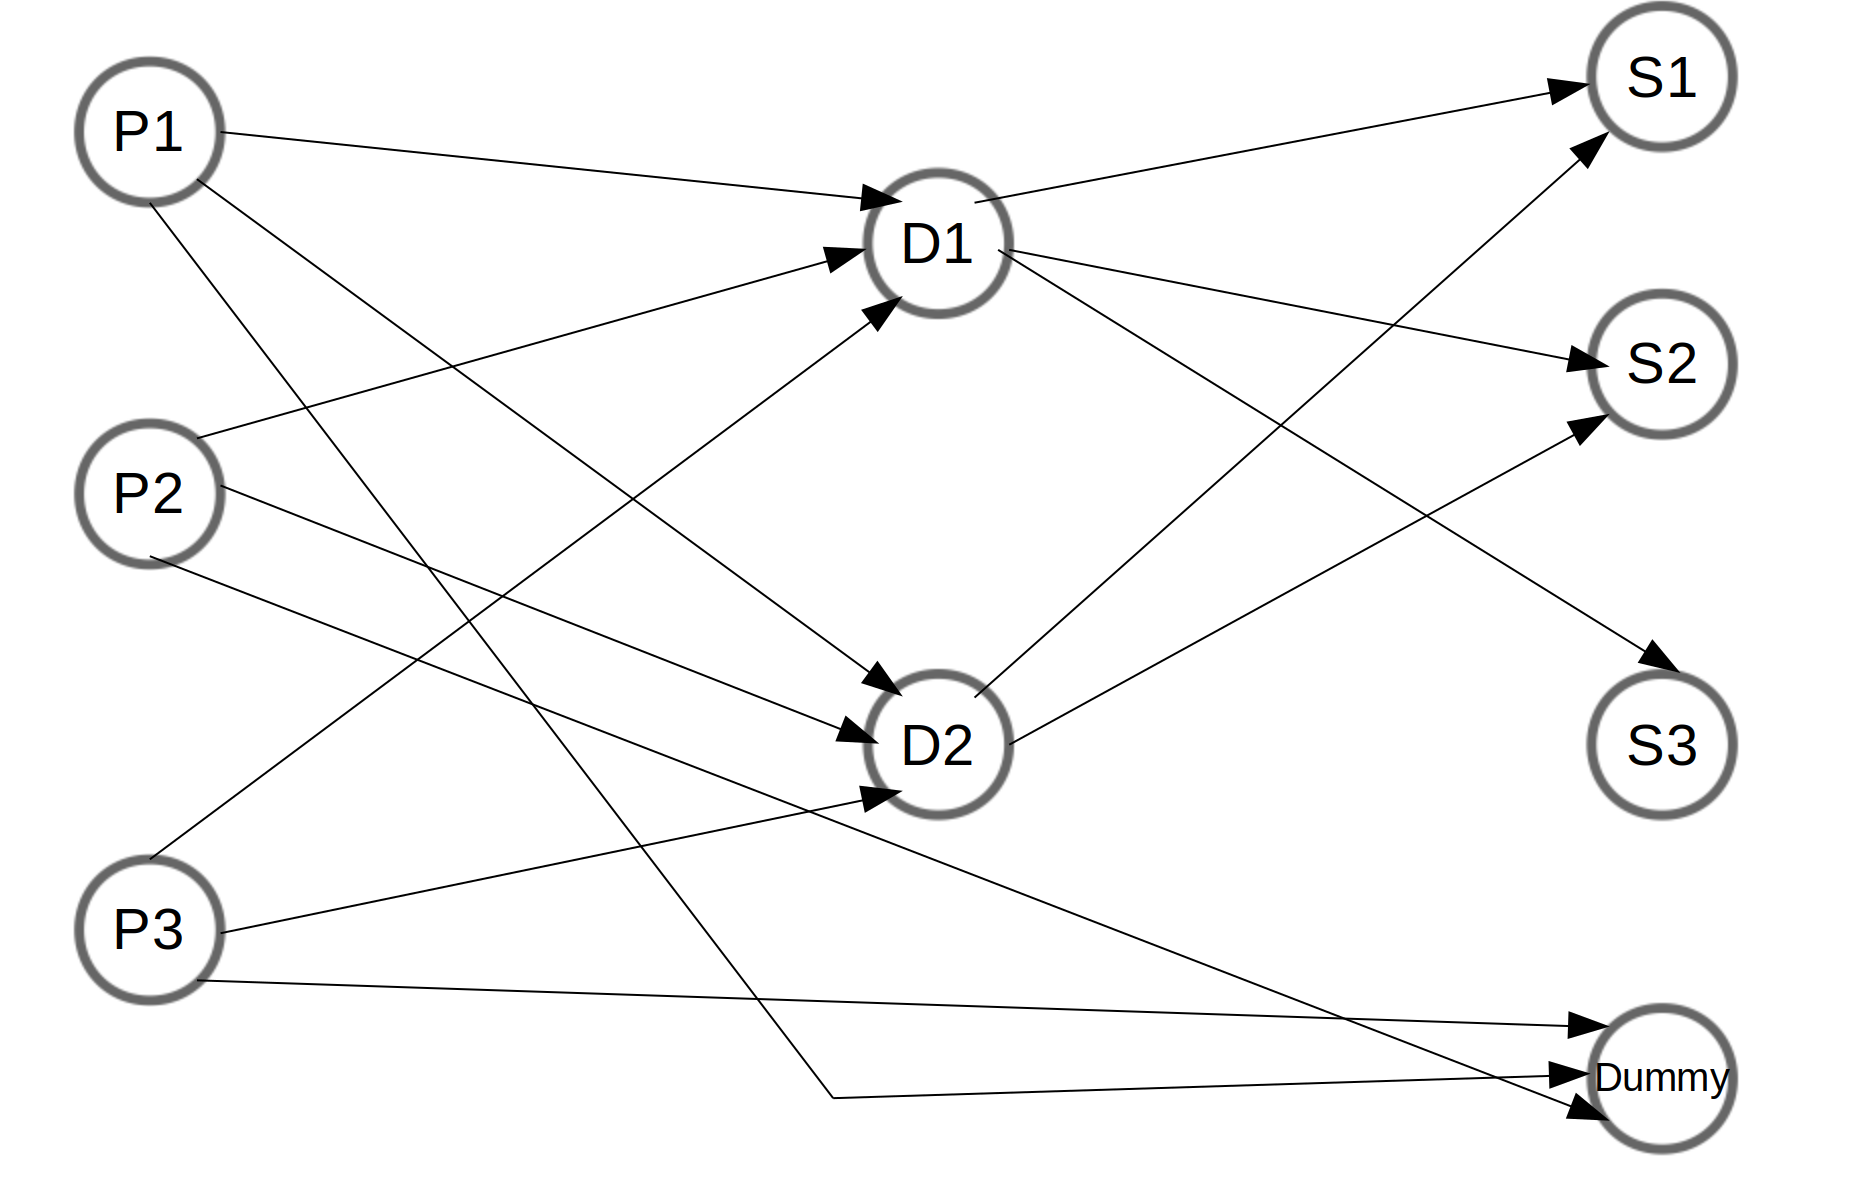
\includegraphics[width=0.9\textwidth]{Prob2.png}
\end{center}

\item[b)] Formulate a concrete model that would allow the brewer to satisfy demand at minimum cost.

{\blu

\textbf{\underline{Decision Variables}}

Let $x_{P1,D1}$ be the number of beer bottles sent from plant 1 to distribution center 1

Let $x_{P1,D2}$ be the number of beer bottles sent from plant 1 to distribution center 2

$\vdots$

Let $x_{D2,S2}$ be the number of beer bottles sent from distribution center 2 to store 2

\textbf{\underline{Objective Function}}

\[
\text{min cost: } 8 x_{P1,D1} + 14 x_{P1,D2} + \cdots + 15 x_{D2,S2} + 0 x_{P1,D} + 0 x_{P2,D} + 0 x_{P3,D}
\]

\textbf{\underline{Constraints}}

\begin{optprog*}
st & x_{P1,D1} + x_{P1,D2} + x_{P1,D} & = & 1000 & \text{(supply of plant 1)} \\
   & x_{P2,D1} + x_{P2,D2} + x_{P1,D} & = & 750  & \text{(supply of plant 2)} \\
   & x_{P3,D1} + x_{P3,D2} + x_{P3,D} & = & 500  & \text{(supply of plant 3)} \\
   & x_{P1,D1} + x_{P2,D1} & = & x_{D1,S1} + x_{D1,S2} + x_{D1,S3} & \text{(flow balance DC 1)} \\   
   & x_{P1,D2} + x_{P2,D2} & = & x_{D2,S1} + x_{D2,S2} + x_{D2,S3} & \text{(flow balance DC 2)} \\
   & x_{D1,S1} + x_{D2,S1} & = & 700 & \text{(demand of store 1)} \\
   & x_{D1,S2} + x_{D2,S2} & = & 600 & \text{(demand of store 2)} \\
   & x_{D1,S3}             & = & 800 & \text{(demand of store 3)} \\
   & x_{P1,D} + x_{P2,D} + x_{P3,D}  & = & 150 & \text{(demand of dummy)} \\
   & x_{P1,D1}, x_{P1,D2}, \hdots, x_{D2,S2} & \geq & 0 \text{ integer} & \text{(non-negativity)}
\end{optprog*}

}


\item[c)] Formulate a parameterized model that would allow the brewer to satisfy demand at minimum cost.
\end{enumerate}

{\blu 

\textbf{\underline{Sets}}

Let $N$ be the set of nodes

Let $E$ be the set of edges

\textbf{\underline{Decision Variables}}

Let $x_{i,j}$ be the number of beer bottles sent along edge $(i,j)$ for all $(i,j) \in E$

\textbf{\underline{Parameters}}

Let $c_{i,j}$ be the cost of edge $(i,j)$ for all $(i,j) \in E$

Let $b_n$ be demand $-$ supply at node $n$ for all $n \in N$


\textbf{\underline{Objective Function}}

\[
\text{min cost: } \sum_{(i,j) \in E} c_{i,j} x_{i,j}
\]

\textbf{\underline{Constraints}}

\begin{optprog*}
st & \sum_{(i,n) \in E} x_{i,n} - \sum_{(n,j) \in E} x_{n,j} = b_n & \text{for all $n \in N$} & \text{(flow balance)} \\
   & x_{i,j} & \in & \mathbb{Z}^+ & \text{for all $(i,j) \in E$} & \text{(non-neg)}
\end{optprog*}
}




\end{document}
